\documentclass[a4paper]{article}

\usepackage[english]{babel}
\usepackage[utf8]{inputenc}
\usepackage{amsmath}
\usepackage{graphicx}
\usepackage[colorinlistoftodos]{todonotes}
\usepackage{amsmath}  
\newtheorem{theorem}{Theorem}  
\newtheorem{definition}{Definition}  
\newtheorem{lemma}{Lemma}  
\newtheorem{proposition}{Proposition}
\newtheorem{proof}{Proof}[section] 
\usepackage{indentfirst}
\usepackage{bbm}
\usepackage{multirow}
\advance\day by -1

\title{Problème de planification culturale durable \footnote{Ce rapport est destiné au TP7 de cours Recherche Opérationnelle et Développement Durable du programme MPRO encadré par Professeur Agnès Plateau sur le sujet de la planification culturale.}}

\author{Ling \textsc{Ma} and Changmin \textsc{Wu}}
\date{\today}

\begin{document}
\maketitle
\tableofcontents

\section{Une représentation du graphe}
Figure \ref{fig:diam} présente un tel graphe dont chaque sommet désigne un état possible de la forme $(l,a,j)$. Un chemin qui commence par $(2,0,0)$ (et de longueur $5$) est donc une rotation de $T=5$ sur la parcelle $p$, par exemple, le chemin $(2,0,0)->(2,1,R)->(2,2,H)->(1,0,0)->(1,1,H)->(1,0,0)$. 
\begin{figure}[h!t]
    \centering
    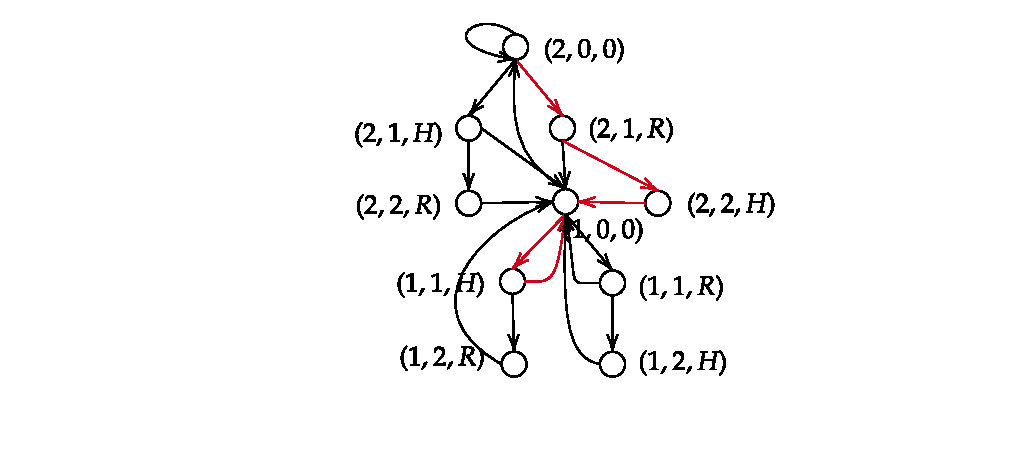
\includegraphics[width=\textwidth]{diagram.pdf}
    \caption{Graphe $G$: les arcs rouges correspondent à une rotation possible; $R$ est \textit{riz} et $H$ est \textit{haricot}}
    \label{fig:diam}
\end{figure}

\section{Modélisation PLNE}
Étant donnée la représentation du graphe, on peut modéliser ce problème de planification comme $P$ problème de flot sur $P$ graphe $G$ qui satisfit une contrainte globale. 
\begin{equation*}
    (P1) \left\{ 
    \begin{aligned}
    \min\quad        & \sum_{p\in P}\sum_{t=1}\sum_{a\in Arc} x_{p,t,a}   \\
    \text{s.t.\quad} & \sum_{p\in P}\sum_{a\in Arc^{-}_{j}} \text{REND}_a x_{p,t,a} \geq D_{j,t} & & \forall t\in \{1, \ldots, T\}, j \in C(s(t)) \\
                     & \sum_{a\in Arc^{-}_{v}} x_{p,t,a} = \sum_{b\in Arc^{+}_{v}} x_{p,t,b} & & \forall t \in \{2, \ldots, T-1\}, p \in \{1, \ldots, P\}, v\in V(G)\\
                     & \sum_{a\in Arc^{-}_{(2,0,0)}} x_{p,1,a} \leq 1 & &  \forall p \in \{1, \ldots, P\} \\
                     & \sum_{a\not\in Arc^{-}_{(2,0,0)}} x_{p,1,a} = 0 & &  \forall p \in \{1, \ldots, P\} \\
                     & x_{p,t,a} \in \{0,1\} & & \forall t \in \{1, \ldots, T\}, p \in \{1, \ldots, P\}, a \in Arcs
  \end{aligned}
\right.
\end{equation*}
où $x_{p,t,a}$ désigne si la transition représentée par $a$ s'effectue au temps $t$ sur la parcelle $p$. $Arc^{-}_{j}$ désigne tous arcs de $G$ incident à $j$ et $Arc^{+}_{j}$ les arcs émergent de $j$. La première contrainte est la contrainte de la demande. La deuxième contrainte est celui de la conservation du flot et les deux prochaines sont les contraintes d'état initial (tout chemin commence de $(2,0,0)$).

\section{Résultat}
Voir tableau \ref{tab:res}.
\begin{table}
    \centering
    \resizebox{1 \textwidth}{!}{
    \begin{tabular}{c|c|c}
    \hline
    Temps de calcul & Nbr Noeuds développés & Nbr Parcelles Cultivées \\
    \hline
    $2.47$s & $1344$ & $19$ \\
    \hline
    \end{tabular}}
    \caption{Information de la solution trouvée}
    \label{tab:res}
\end{table}

\section{Une ré-formulation}
Supposons que les rotations $r$ sont énumérable, on a
\begin{equation*}
    (P2) \left\{ 
    \begin{aligned}
    \min\quad        & \sum_{r \in R} x_{r}   \\
    \text{s.t.\quad} & \sum_{r \in R} \text{REND}_{r_t = } x_{r} \geq D_{j,t} & & \forall t\in \{1, \ldots, T\}, j \in C(s(t))\\
                     & x_i \in \{0,1\}            & & i\in N
  \end{aligned}
\right.
\end{equation*}
\section{Génération du colonnes}
\end{document}
